% Options for packages loaded elsewhere
\PassOptionsToPackage{unicode}{hyperref}
\PassOptionsToPackage{hyphens}{url}
%
\documentclass[
]{article}
\usepackage{amsmath,amssymb}
\usepackage{iftex}
\ifPDFTeX
  \usepackage[T1]{fontenc}
  \usepackage[utf8]{inputenc}
  \usepackage{textcomp} % provide euro and other symbols
\else % if luatex or xetex
  \usepackage{unicode-math} % this also loads fontspec
  \defaultfontfeatures{Scale=MatchLowercase}
  \defaultfontfeatures[\rmfamily]{Ligatures=TeX,Scale=1}
\fi
\usepackage{lmodern}
\ifPDFTeX\else
  % xetex/luatex font selection
\fi
% Use upquote if available, for straight quotes in verbatim environments
\IfFileExists{upquote.sty}{\usepackage{upquote}}{}
\IfFileExists{microtype.sty}{% use microtype if available
  \usepackage[]{microtype}
  \UseMicrotypeSet[protrusion]{basicmath} % disable protrusion for tt fonts
}{}
\makeatletter
\@ifundefined{KOMAClassName}{% if non-KOMA class
  \IfFileExists{parskip.sty}{%
    \usepackage{parskip}
  }{% else
    \setlength{\parindent}{0pt}
    \setlength{\parskip}{6pt plus 2pt minus 1pt}}
}{% if KOMA class
  \KOMAoptions{parskip=half}}
\makeatother
\usepackage{xcolor}
\usepackage[margin=1in]{geometry}
\usepackage{color}
\usepackage{fancyvrb}
\newcommand{\VerbBar}{|}
\newcommand{\VERB}{\Verb[commandchars=\\\{\}]}
\DefineVerbatimEnvironment{Highlighting}{Verbatim}{commandchars=\\\{\}}
% Add ',fontsize=\small' for more characters per line
\usepackage{framed}
\definecolor{shadecolor}{RGB}{248,248,248}
\newenvironment{Shaded}{\begin{snugshade}}{\end{snugshade}}
\newcommand{\AlertTok}[1]{\textcolor[rgb]{0.94,0.16,0.16}{#1}}
\newcommand{\AnnotationTok}[1]{\textcolor[rgb]{0.56,0.35,0.01}{\textbf{\textit{#1}}}}
\newcommand{\AttributeTok}[1]{\textcolor[rgb]{0.13,0.29,0.53}{#1}}
\newcommand{\BaseNTok}[1]{\textcolor[rgb]{0.00,0.00,0.81}{#1}}
\newcommand{\BuiltInTok}[1]{#1}
\newcommand{\CharTok}[1]{\textcolor[rgb]{0.31,0.60,0.02}{#1}}
\newcommand{\CommentTok}[1]{\textcolor[rgb]{0.56,0.35,0.01}{\textit{#1}}}
\newcommand{\CommentVarTok}[1]{\textcolor[rgb]{0.56,0.35,0.01}{\textbf{\textit{#1}}}}
\newcommand{\ConstantTok}[1]{\textcolor[rgb]{0.56,0.35,0.01}{#1}}
\newcommand{\ControlFlowTok}[1]{\textcolor[rgb]{0.13,0.29,0.53}{\textbf{#1}}}
\newcommand{\DataTypeTok}[1]{\textcolor[rgb]{0.13,0.29,0.53}{#1}}
\newcommand{\DecValTok}[1]{\textcolor[rgb]{0.00,0.00,0.81}{#1}}
\newcommand{\DocumentationTok}[1]{\textcolor[rgb]{0.56,0.35,0.01}{\textbf{\textit{#1}}}}
\newcommand{\ErrorTok}[1]{\textcolor[rgb]{0.64,0.00,0.00}{\textbf{#1}}}
\newcommand{\ExtensionTok}[1]{#1}
\newcommand{\FloatTok}[1]{\textcolor[rgb]{0.00,0.00,0.81}{#1}}
\newcommand{\FunctionTok}[1]{\textcolor[rgb]{0.13,0.29,0.53}{\textbf{#1}}}
\newcommand{\ImportTok}[1]{#1}
\newcommand{\InformationTok}[1]{\textcolor[rgb]{0.56,0.35,0.01}{\textbf{\textit{#1}}}}
\newcommand{\KeywordTok}[1]{\textcolor[rgb]{0.13,0.29,0.53}{\textbf{#1}}}
\newcommand{\NormalTok}[1]{#1}
\newcommand{\OperatorTok}[1]{\textcolor[rgb]{0.81,0.36,0.00}{\textbf{#1}}}
\newcommand{\OtherTok}[1]{\textcolor[rgb]{0.56,0.35,0.01}{#1}}
\newcommand{\PreprocessorTok}[1]{\textcolor[rgb]{0.56,0.35,0.01}{\textit{#1}}}
\newcommand{\RegionMarkerTok}[1]{#1}
\newcommand{\SpecialCharTok}[1]{\textcolor[rgb]{0.81,0.36,0.00}{\textbf{#1}}}
\newcommand{\SpecialStringTok}[1]{\textcolor[rgb]{0.31,0.60,0.02}{#1}}
\newcommand{\StringTok}[1]{\textcolor[rgb]{0.31,0.60,0.02}{#1}}
\newcommand{\VariableTok}[1]{\textcolor[rgb]{0.00,0.00,0.00}{#1}}
\newcommand{\VerbatimStringTok}[1]{\textcolor[rgb]{0.31,0.60,0.02}{#1}}
\newcommand{\WarningTok}[1]{\textcolor[rgb]{0.56,0.35,0.01}{\textbf{\textit{#1}}}}
\usepackage{graphicx}
\makeatletter
\newsavebox\pandoc@box
\newcommand*\pandocbounded[1]{% scales image to fit in text height/width
  \sbox\pandoc@box{#1}%
  \Gscale@div\@tempa{\textheight}{\dimexpr\ht\pandoc@box+\dp\pandoc@box\relax}%
  \Gscale@div\@tempb{\linewidth}{\wd\pandoc@box}%
  \ifdim\@tempb\p@<\@tempa\p@\let\@tempa\@tempb\fi% select the smaller of both
  \ifdim\@tempa\p@<\p@\scalebox{\@tempa}{\usebox\pandoc@box}%
  \else\usebox{\pandoc@box}%
  \fi%
}
% Set default figure placement to htbp
\def\fps@figure{htbp}
\makeatother
\ifLuaTeX
  \usepackage{luacolor}
  \usepackage[soul]{lua-ul}
\else
  \usepackage{soul}
\fi
\setlength{\emergencystretch}{3em} % prevent overfull lines
\providecommand{\tightlist}{%
  \setlength{\itemsep}{0pt}\setlength{\parskip}{0pt}}
\setcounter{secnumdepth}{5}
\usepackage{bookmark}
\IfFileExists{xurl.sty}{\usepackage{xurl}}{} % add URL line breaks if available
\urlstyle{same}
\hypersetup{
  pdftitle={Simple Linear Regression},
  pdfauthor={Allan Omondi},
  hidelinks,
  pdfcreator={LaTeX via pandoc}}

\title{Simple Linear Regression}
\author{Allan Omondi}
\date{2025-05-27}

\begin{document}
\maketitle

{
\setcounter{tocdepth}{4}
\tableofcontents
}
\begin{Shaded}
\begin{Highlighting}[]
\NormalTok{knitr}\SpecialCharTok{::}\NormalTok{opts\_chunk}\SpecialCharTok{$}\FunctionTok{set}\NormalTok{(}\AttributeTok{echo =} \ConstantTok{TRUE}\NormalTok{)}
\CommentTok{\# \textasciigrave{}installed.packages()\textasciigrave{} retrieves a matrix of all installed packages}
\CommentTok{\# \textasciigrave{}[, "Package"]\textasciigrave{} extracts on the "Package" column from the matrix of all packages}
\CommentTok{\# The \%in\% operator is used to test if the specified package is in the matrix of all packages}
\CommentTok{\# \textasciigrave{}character.only = TRUE\textasciigrave{} ensures that the quoted name of the package is not treated as a symbol}
\CommentTok{\# \textasciigrave{}dependencies = TRUE\textasciigrave{} instructs R to install not only the specified package but also its dependencies}
\CommentTok{\# \textasciigrave{}knitr::opts\_knit$set(root.dir = here::here())\textasciigrave{} is used to ensure that the "knitr" utility in R knows where to find the files required to create the HTML, Word, or PDF version of the notebook.}

\ControlFlowTok{if}\NormalTok{ (}\SpecialCharTok{!}\StringTok{"pacman"} \SpecialCharTok{\%in\%} \FunctionTok{installed.packages}\NormalTok{()[, }\StringTok{"Package"}\NormalTok{]) \{}
  \FunctionTok{install.packages}\NormalTok{(}\StringTok{"pacman"}\NormalTok{, }\AttributeTok{dependencies =} \ConstantTok{TRUE}\NormalTok{)}
  \FunctionTok{library}\NormalTok{(}\StringTok{"pacman"}\NormalTok{, }\AttributeTok{character.only =} \ConstantTok{TRUE}\NormalTok{)}
\NormalTok{\}}

\NormalTok{pacman}\SpecialCharTok{::}\FunctionTok{p\_load}\NormalTok{(}\StringTok{"here"}\NormalTok{)}

\NormalTok{knitr}\SpecialCharTok{::}\NormalTok{opts\_knit}\SpecialCharTok{$}\FunctionTok{set}\NormalTok{(}\AttributeTok{root.dir =}\NormalTok{ here}\SpecialCharTok{::}\FunctionTok{here}\NormalTok{())}
\end{Highlighting}
\end{Shaded}

\section{Load the Dataset}\label{load-the-dataset}

The following synthetic dataset contains the estimated Customer Lifetime
Value (CLV) as the dependent variable and the customer purchase
frequency as the independent variable. The dataset is loaded as shown
below.

\begin{Shaded}
\begin{Highlighting}[]
\CommentTok{\# \textasciigrave{}pacman::p\_load()\textasciigrave{} is designed to both install and load packages}
\NormalTok{pacman}\SpecialCharTok{::}\FunctionTok{p\_load}\NormalTok{(}\StringTok{"readr"}\NormalTok{)}

\NormalTok{clv\_data }\OtherTok{\textless{}{-}} \FunctionTok{read\_csv}\NormalTok{(}\StringTok{"./data/clv\_data.csv"}\NormalTok{)}
\FunctionTok{head}\NormalTok{(clv\_data)}
\end{Highlighting}
\end{Shaded}

\begin{verbatim}
## # A tibble: 6 x 2
##   purchase_frequency customer_lifetime_value
##                <dbl>                   <dbl>
## 1                  3                   110. 
## 2                  7                   190. 
## 3                  6                   160. 
## 4                  2                    94.4
## 5                  4                   133. 
## 6                  8                   223.
\end{verbatim}

\section{Initial EDA}\label{initial-eda}

\ul{\textbf{View the Dimensions}}

The number of observations and the number of variables.

\begin{Shaded}
\begin{Highlighting}[]
\FunctionTok{dim}\NormalTok{(clv\_data)}
\end{Highlighting}
\end{Shaded}

\begin{verbatim}
## [1] 500   2
\end{verbatim}

\ul{\textbf{View the Data Types}}

\begin{Shaded}
\begin{Highlighting}[]
\FunctionTok{sapply}\NormalTok{(clv\_data, class)}
\end{Highlighting}
\end{Shaded}

\begin{verbatim}
##      purchase_frequency customer_lifetime_value 
##               "numeric"               "numeric"
\end{verbatim}

\begin{Shaded}
\begin{Highlighting}[]
\FunctionTok{str}\NormalTok{(clv\_data)}
\end{Highlighting}
\end{Shaded}

\begin{verbatim}
## spc_tbl_ [500 x 2] (S3: spec_tbl_df/tbl_df/tbl/data.frame)
##  $ purchase_frequency     : num [1:500] 3 7 6 2 4 8 0 4 8 3 ...
##  $ customer_lifetime_value: num [1:500] 110.3 190.2 160 94.4 133.2 ...
##  - attr(*, "spec")=
##   .. cols(
##   ..   purchase_frequency = col_double(),
##   ..   customer_lifetime_value = col_double()
##   .. )
##  - attr(*, "problems")=<externalptr>
\end{verbatim}

\ul{\textbf{Descriptive Statistics}}

Understanding your data can lead to:

\begin{itemize}
\item
  \textbf{Data cleaning:} To remove extreme outliers or impute missing
  data.
\item
  \textbf{Data transformation:} To reduce skewness
\item
  \textbf{Data modelling:} You may notice properties of the data such as
  distributions or data types that suggest the use of parametric or
  non-parametric statistical tests and algorithms
\end{itemize}

Descriptive statistics can be used to understand your data. Typical
descriptive statistics include:

\begin{enumerate}
\def\labelenumi{\arabic{enumi}.}
\item
  \textbf{Measures of frequency:} count and percent
\item
  \textbf{Measures of central tendency:} mean, median, and mode
\item
  \textbf{Measures of
  distribution/dispersion/spread/scatter/variability:} minimum,
  quartiles, maximum, variance, standard deviation, coefficient of
  variation, range, interquartile range (IQR) {[}includes a box and
  whisker plot for visualization{]}, kurtosis, skewness {[}includes a
  histogram for visualization{]}).
\item
  \textbf{Measures of relationship:} covariance and correlation
\end{enumerate}

\subsection{\texorpdfstring{\ul{\textbf{Measures of
Frequency}}}{Measures of Frequency}}\label{measures-of-frequency}

This is applicable in cases where you have categorical variables, e.g.,
60\% of the observations are male and 40\% are female (2 categories).

\subsection{\texorpdfstring{\ul{\textbf{Measures of Central
Tendency}}}{Measures of Central Tendency}}\label{measures-of-central-tendency}

The median and the mean of each numeric variable:

\begin{Shaded}
\begin{Highlighting}[]
\FunctionTok{summary}\NormalTok{(clv\_data)}
\end{Highlighting}
\end{Shaded}

\begin{verbatim}
##  purchase_frequency customer_lifetime_value
##  Min.   :-1.000     Min.   : 26.13         
##  1st Qu.: 4.000     1st Qu.:122.04         
##  Median : 5.000     Median :148.21         
##  Mean   : 4.914     Mean   :148.25         
##  3rd Qu.: 6.000     3rd Qu.:175.88         
##  Max.   :11.000     Max.   :262.04
\end{verbatim}

\subsection{\texorpdfstring{\ul{\textbf{Measures of
Distribution}}}{Measures of Distribution}}\label{measures-of-distribution}

Measuring the variability in the dataset is important because the amount
of variability determines \textbf{how well you can generalize} results
from the sample to a new observation in the population.

Low variability is ideal because it means that you can better predict
information about the population based on the sample data. High
variability means that the values are less consistent, thus making it
harder to make predictions.

The syntax \texttt{dataset{[}rows,\ columns{]}} can be used to specify
the exact rows and columns to be considered.
\texttt{dataset{[},\ columns{]}} implies all rows will be considered.
For example, specifying \texttt{BostonHousing{[},\ -4{]}} implies all
the columns except column number 4. This can also be stated as
\texttt{BostonHousing{[},\ c(1,2,3,5,6,7,8,9,10,11,12,13,14){]}}. This
allows us to calculate the standard deviation of only columns that are
numeric, thus leaving out the columns termed as ``factors''
(categorical) or those that have a string data type.

\subsubsection{\texorpdfstring{\textbf{Variance}}{Variance}}\label{variance}

\begin{Shaded}
\begin{Highlighting}[]
\CommentTok{\# \textasciigrave{}sapply()\textasciigrave{} is designed to apply a function to a variable in a dataset}
\CommentTok{\# In this case, we use \textasciigrave{}sapply()\textasciigrave{} to apply the \textasciigrave{}var()\textasciigrave{} function used to compute the variance.}
\FunctionTok{sapply}\NormalTok{(clv\_data[,], var)}
\end{Highlighting}
\end{Shaded}

\begin{verbatim}
##      purchase_frequency customer_lifetime_value 
##                4.146898             1642.315996
\end{verbatim}

\subsubsection{\texorpdfstring{\textbf{Standard
Deviation}}{Standard Deviation}}\label{standard-deviation}

\begin{Shaded}
\begin{Highlighting}[]
\FunctionTok{sapply}\NormalTok{(clv\_data[,], sd)}
\end{Highlighting}
\end{Shaded}

\begin{verbatim}
##      purchase_frequency customer_lifetime_value 
##                2.036393               40.525498
\end{verbatim}

\subsubsection{\texorpdfstring{\textbf{Kurtosis}}{Kurtosis}}\label{kurtosis}

The Kurtosis informs us of how often outliers occur in the results.
There are different formulas for calculating kurtosis. Specifying ``type
= 2'' allows us to use the 2nd formula which is the same kurtosis
formula used in other statistical software like SPSS and SAS.

In ``type = 2'' (used in SPSS and SAS):

\begin{enumerate}
\def\labelenumi{\arabic{enumi}.}
\item
  Kurtosis \textless{} 3 implies a low number of outliers
\item
  Kurtosis = 3 implies a medium number of outliers
\item
  Kurtosis \textgreater{} 3 implies a high number of outliers
\end{enumerate}

\begin{Shaded}
\begin{Highlighting}[]
\NormalTok{pacman}\SpecialCharTok{::}\FunctionTok{p\_load}\NormalTok{(}\StringTok{"e1071"}\NormalTok{)}
\FunctionTok{sapply}\NormalTok{(clv\_data[,],  kurtosis, }\AttributeTok{type =} \DecValTok{2}\NormalTok{)}
\end{Highlighting}
\end{Shaded}

\begin{verbatim}
##      purchase_frequency customer_lifetime_value 
##              -0.1220038              -0.1484811
\end{verbatim}

\subsubsection{\texorpdfstring{\textbf{Skewness}}{Skewness}}\label{skewness}

The skewness is used to identify the asymmetry of the distribution of
results. Similar to kurtosis, there are several ways of computing the
skewness.

Using ``type = 2'' (common in other statistical software like SPSS and
SAS) can be interpreted as:

\begin{enumerate}
\def\labelenumi{\arabic{enumi}.}
\item
  Skewness between -0.4 and 0.4 (inclusive) implies that there is no
  skew in the distribution of results; the distribution of results is
  symmetrical; it is a normal distribution; a Gaussian distribution.
\item
  Skewness above 0.4 implies a positive skew; a right-skewed
  distribution.
\item
  Skewness below -0.4 implies a negative skew; a left-skewed
  distribution.
\end{enumerate}

\begin{Shaded}
\begin{Highlighting}[]
\FunctionTok{sapply}\NormalTok{(clv\_data[,], skewness, }\AttributeTok{type =} \DecValTok{2}\NormalTok{)}
\end{Highlighting}
\end{Shaded}

\begin{verbatim}
##      purchase_frequency customer_lifetime_value 
##             -0.04021915             -0.01608242
\end{verbatim}

\subsection{\texorpdfstring{\ul{\textbf{Measures of
Relationship}}}{Measures of Relationship}}\label{measures-of-relationship}

\subsubsection{\texorpdfstring{\textbf{Covariance}}{Covariance}}\label{covariance}

Covariance is a statistical measure that indicates the direction of the
linear relationship between two variables. It assesses whether increases
in one variable correspond to increases or decreases in
another.\hspace{0pt}

\begin{itemize}
\item
  \textbf{Positive Covariance:} When one variable increases, the other
  tends to increase as well.
\item
  \textbf{Negative Covariance:} When one variable increases, the other
  tends to decrease.
\item
  \textbf{Zero Covariance:} No linear relationship exists between the
  variables.
\end{itemize}

While covariance indicates the direction of a relationship, it does not
convey the strength or consistency of the relationship. The correlation
coefficient is used to indicate the strength of the relationship.

\begin{Shaded}
\begin{Highlighting}[]
\FunctionTok{cov}\NormalTok{(clv\_data, }\AttributeTok{method =} \StringTok{"spearman"}\NormalTok{)}
\end{Highlighting}
\end{Shaded}

\begin{verbatim}
##                         purchase_frequency customer_lifetime_value
## purchase_frequency                20409.91                20235.73
## customer_lifetime_value           20235.73                20874.99
\end{verbatim}

\subsubsection{\texorpdfstring{\textbf{Correlation}}{Correlation}}\label{correlation}

A strong correlation between variables enables us to better predict the
value of the dependent variable using the value of the independent
variable. However, a weak correlation between two variables does not
help us to predict the value of the dependent variable from the value of
the independent variable. This is useful only if there is a linear
association between the variables.

We can measure the statistical significance of the correlation using
Spearman's rank correlation \emph{rho}. This shows us if the variables
are significantly monotonically related. A monotonic relationship
between two variables implies that as one variable increases, the other
variable either consistently increases or consistently decreases. The
key characteristic is the preservation of the direction of change,
though the rate of change may vary.

\begin{Shaded}
\begin{Highlighting}[]
\FunctionTok{cor.test}\NormalTok{(clv\_data}\SpecialCharTok{$}\NormalTok{customer\_lifetime\_value, clv\_data}\SpecialCharTok{$}\NormalTok{purchase\_frequency, }\AttributeTok{method =} \StringTok{"spearman"}\NormalTok{)}
\end{Highlighting}
\end{Shaded}

\begin{verbatim}
## 
##  Spearman's rank correlation rho
## 
## data:  clv_data$customer_lifetime_value and clv_data$purchase_frequency
## S = 409190, p-value < 2.2e-16
## alternative hypothesis: true rho is not equal to 0
## sample estimates:
##       rho 
## 0.9803588
\end{verbatim}

To view the correlation of all variables

\begin{Shaded}
\begin{Highlighting}[]
\FunctionTok{cor}\NormalTok{(clv\_data, }\AttributeTok{method =} \StringTok{"spearman"}\NormalTok{)}
\end{Highlighting}
\end{Shaded}

\begin{verbatim}
##                         purchase_frequency customer_lifetime_value
## purchase_frequency               1.0000000               0.9803588
## customer_lifetime_value          0.9803588               1.0000000
\end{verbatim}

\subsection{\texorpdfstring{\ul{\textbf{Basic
Visualizations}}}{Basic Visualizations}}\label{basic-visualizations}

\subsubsection{\texorpdfstring{\textbf{Histogram}}{Histogram}}\label{histogram}

\begin{Shaded}
\begin{Highlighting}[]
\CommentTok{\# \textasciigrave{}par(mfrow = c(1, 2))\textasciigrave{} This is used to divide the area used to plot}
\CommentTok{\# the visualization into a 1 row by 2 columns grid}
\CommentTok{\# \textasciigrave{}for (i in 1:2)\textasciigrave{} This is used to identify the variable (column) }
\CommentTok{\# that is being processed}
\CommentTok{\# \textasciigrave{}clv\_data[[i]]\textasciigrave{} This is used to extract the i{-}th column as a vector}
\CommentTok{\# \textasciigrave{}hist()\textasciigrave{} This is the function used to plot the histogram}
\FunctionTok{par}\NormalTok{(}\AttributeTok{mfrow =} \FunctionTok{c}\NormalTok{(}\DecValTok{1}\NormalTok{, }\DecValTok{2}\NormalTok{))}
\ControlFlowTok{for}\NormalTok{ (i }\ControlFlowTok{in} \DecValTok{1}\SpecialCharTok{:}\DecValTok{2}\NormalTok{) \{}
  \ControlFlowTok{if}\NormalTok{ (}\FunctionTok{is.numeric}\NormalTok{(clv\_data[[i]])) \{}
    \FunctionTok{hist}\NormalTok{(clv\_data[[i]],}
         \AttributeTok{main =} \FunctionTok{names}\NormalTok{(clv\_data)[i],}
         \AttributeTok{xlab =} \FunctionTok{names}\NormalTok{(clv\_data)[i])}
\NormalTok{  \} }\ControlFlowTok{else}\NormalTok{ \{}
    \FunctionTok{message}\NormalTok{(}\FunctionTok{paste}\NormalTok{(}\StringTok{"Column"}\NormalTok{, }\FunctionTok{names}\NormalTok{(clv\_data)[i],}
                  \StringTok{"is not numeric and will be skipped."}\NormalTok{))}
\NormalTok{  \}}
\NormalTok{\}}
\end{Highlighting}
\end{Shaded}

\pandocbounded{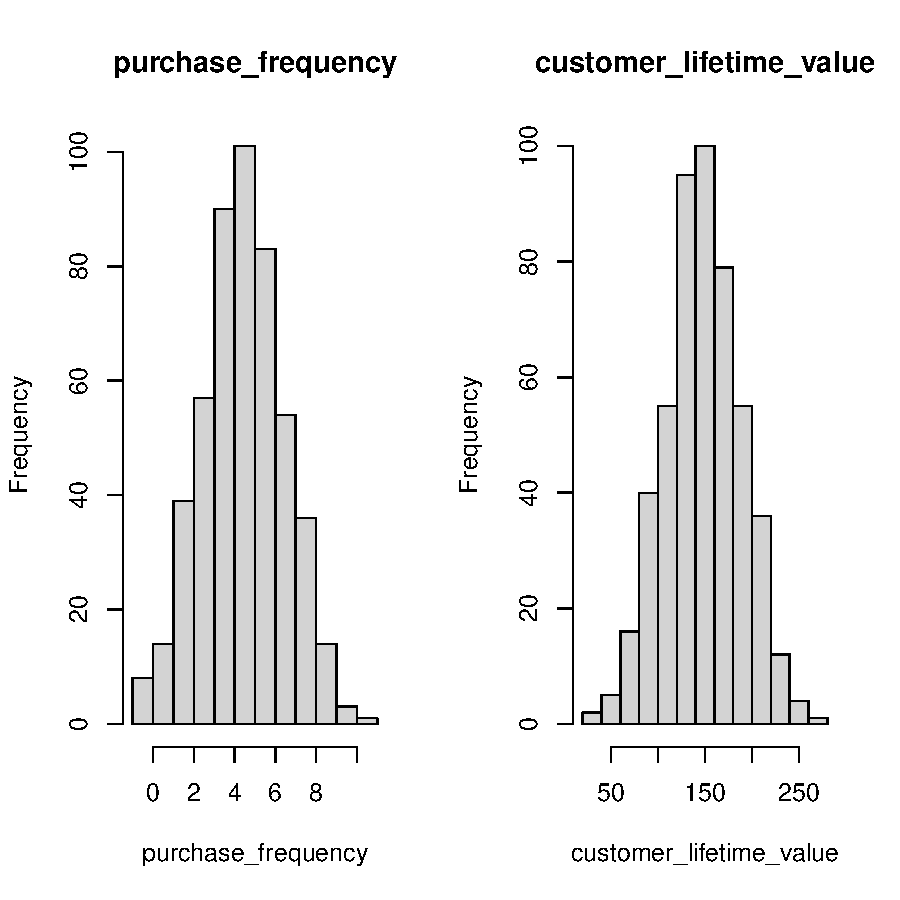
\includegraphics[keepaspectratio]{1_simple_linear_regression_files/figure-latex/visualization_histogram-1.pdf}}

\subsubsection{\texorpdfstring{\textbf{Box and Whisker
Plot}}{Box and Whisker Plot}}\label{box-and-whisker-plot}

\begin{Shaded}
\begin{Highlighting}[]
\CommentTok{\# \textasciigrave{}boxplot()\textasciigrave{} This is the function used to plot the box and whisker plot visualization}
\FunctionTok{par}\NormalTok{(}\AttributeTok{mfrow =} \FunctionTok{c}\NormalTok{(}\DecValTok{1}\NormalTok{, }\DecValTok{2}\NormalTok{))}
\ControlFlowTok{for}\NormalTok{ (i }\ControlFlowTok{in} \DecValTok{1}\SpecialCharTok{:}\DecValTok{2}\NormalTok{) \{}
  \ControlFlowTok{if}\NormalTok{ (}\FunctionTok{is.numeric}\NormalTok{(clv\_data[[i]])) \{}
    \FunctionTok{boxplot}\NormalTok{(clv\_data[[i]], }\AttributeTok{main =} \FunctionTok{names}\NormalTok{(clv\_data)[i])}
\NormalTok{  \} }\ControlFlowTok{else}\NormalTok{ \{}
    \FunctionTok{message}\NormalTok{(}\FunctionTok{paste}\NormalTok{(}\StringTok{"Column"}\NormalTok{, }\FunctionTok{names}\NormalTok{(clv\_data)[i], }\StringTok{"is not numeric and will be skipped."}\NormalTok{))}
\NormalTok{  \}}
\NormalTok{\}}
\end{Highlighting}
\end{Shaded}

\pandocbounded{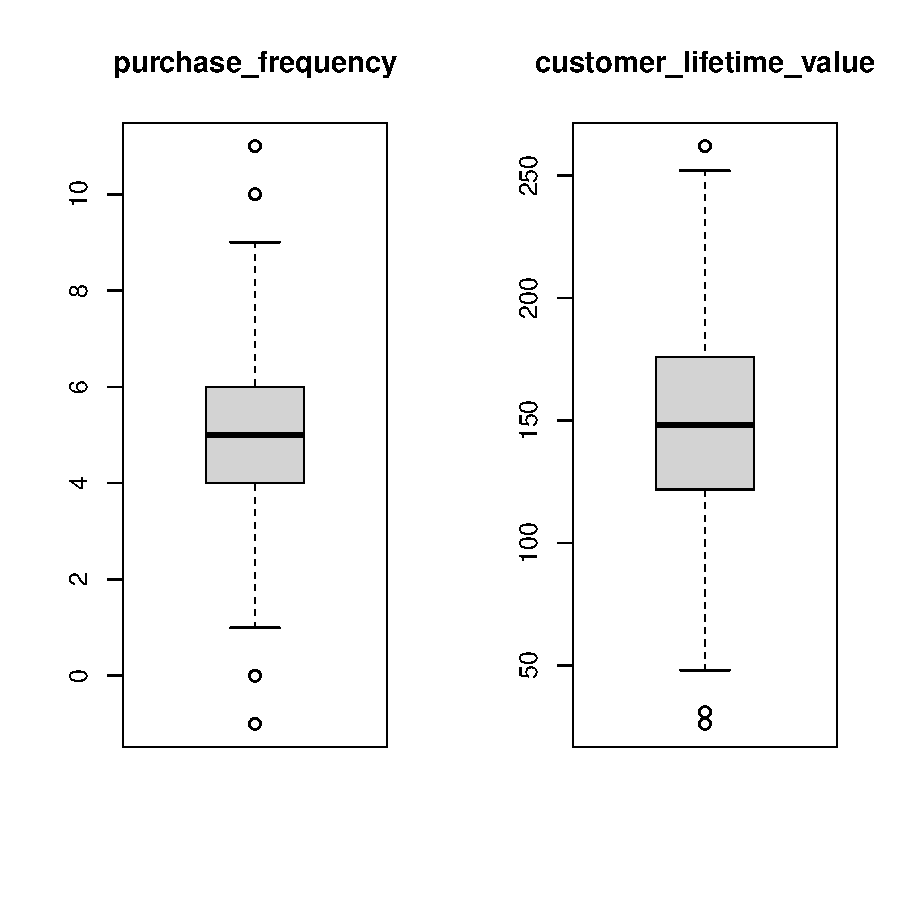
\includegraphics[keepaspectratio]{1_simple_linear_regression_files/figure-latex/visualization_boxplot-1.pdf}}

\subsubsection{\texorpdfstring{\textbf{Missing Data
Plot}}{Missing Data Plot}}\label{missing-data-plot}

\begin{Shaded}
\begin{Highlighting}[]
\NormalTok{pacman}\SpecialCharTok{::}\FunctionTok{p\_load}\NormalTok{(}\StringTok{"Amelia"}\NormalTok{)}

\FunctionTok{missmap}\NormalTok{(clv\_data, }\AttributeTok{col =} \FunctionTok{c}\NormalTok{(}\StringTok{"red"}\NormalTok{, }\StringTok{"grey"}\NormalTok{), }\AttributeTok{legend =} \ConstantTok{TRUE}\NormalTok{)}
\end{Highlighting}
\end{Shaded}

\pandocbounded{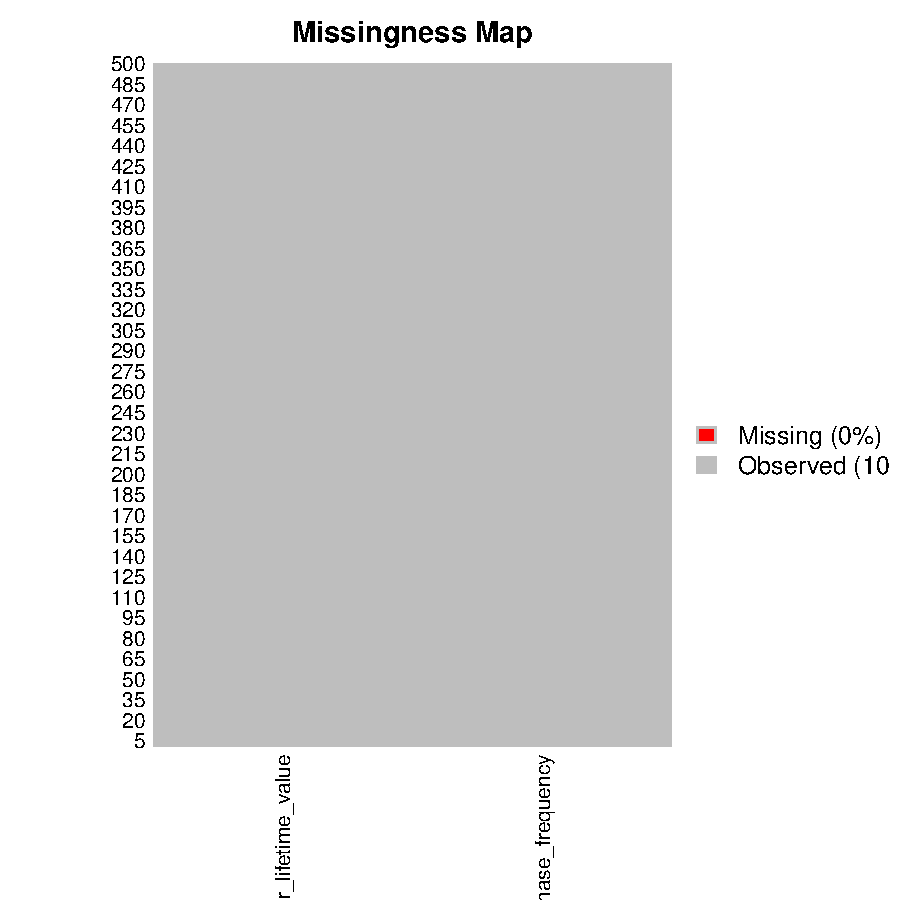
\includegraphics[keepaspectratio]{1_simple_linear_regression_files/figure-latex/missing_data_plot-1.pdf}}

\subsubsection{\texorpdfstring{\textbf{Correlation
Plot}}{Correlation Plot}}\label{correlation-plot}

\begin{Shaded}
\begin{Highlighting}[]
\NormalTok{pacman}\SpecialCharTok{::}\FunctionTok{p\_load}\NormalTok{(}\StringTok{"ggcorrplot"}\NormalTok{)}

\FunctionTok{ggcorrplot}\NormalTok{(}\FunctionTok{cor}\NormalTok{(clv\_data[,]))}
\end{Highlighting}
\end{Shaded}

\pandocbounded{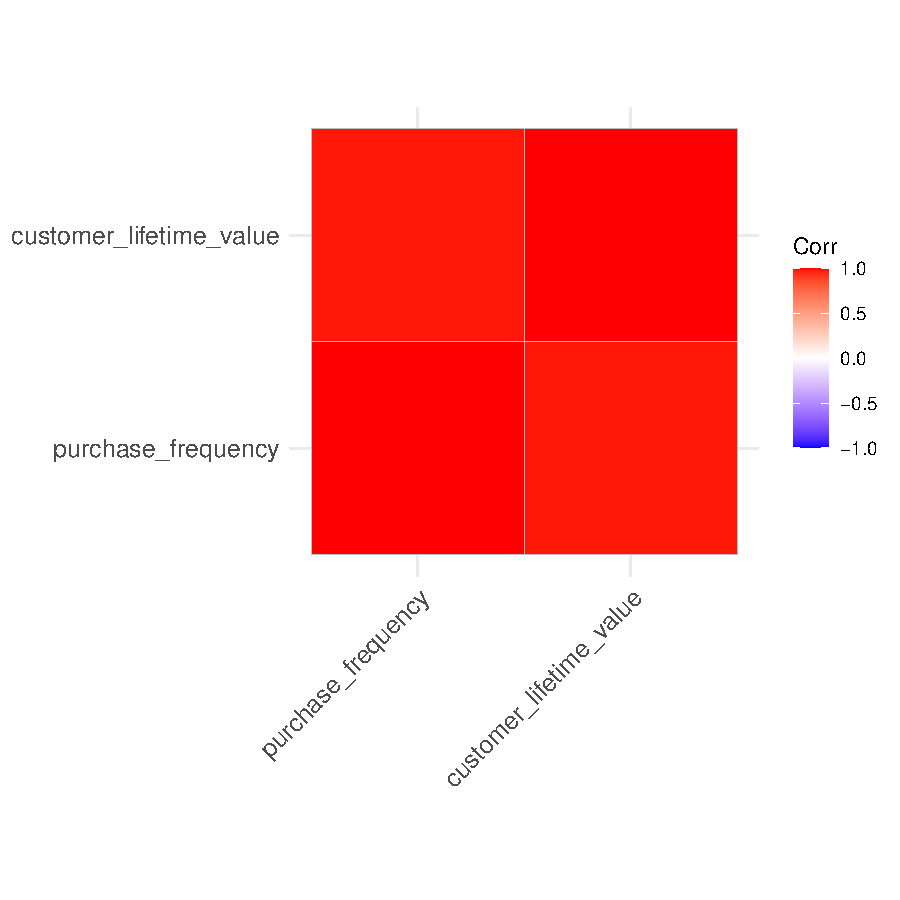
\includegraphics[keepaspectratio]{1_simple_linear_regression_files/figure-latex/correlation_plot-1.pdf}}

\subsubsection{\texorpdfstring{\textbf{Scatter
Plot}}{Scatter Plot}}\label{scatter-plot}

\begin{Shaded}
\begin{Highlighting}[]
\NormalTok{pacman}\SpecialCharTok{::}\FunctionTok{p\_load}\NormalTok{(}\StringTok{"corrplot"}\NormalTok{)}

\FunctionTok{pairs}\NormalTok{(customer\_lifetime\_value }\SpecialCharTok{\textasciitilde{}}\NormalTok{ ., }\AttributeTok{data =}\NormalTok{ clv\_data,}
      \AttributeTok{col =}\NormalTok{ clv\_data}\SpecialCharTok{$}\NormalTok{customer\_lifetime\_value)}
\end{Highlighting}
\end{Shaded}

\pandocbounded{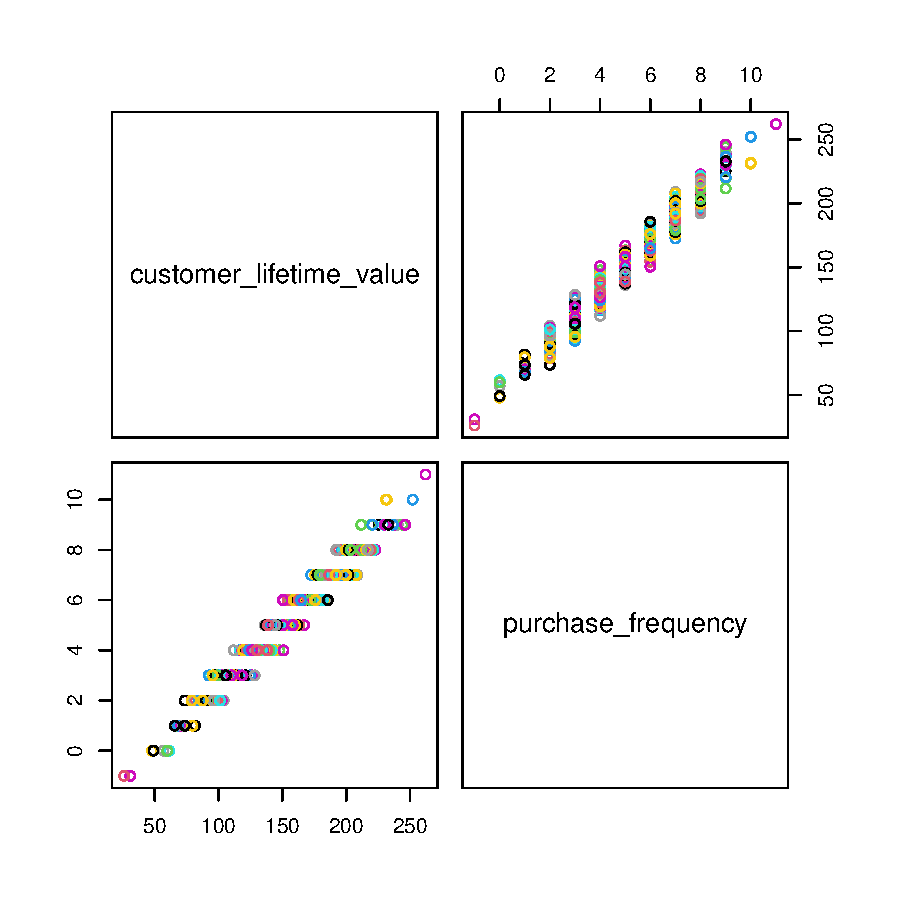
\includegraphics[keepaspectratio]{1_simple_linear_regression_files/figure-latex/scatter_plot_1-1.pdf}}

\begin{Shaded}
\begin{Highlighting}[]
\NormalTok{pacman}\SpecialCharTok{::}\FunctionTok{p\_load}\NormalTok{(}\StringTok{"ggplot2"}\NormalTok{)}
\FunctionTok{ggplot}\NormalTok{(clv\_data,}
       \FunctionTok{aes}\NormalTok{(}\AttributeTok{x =}\NormalTok{ purchase\_frequency, }\AttributeTok{y =}\NormalTok{ customer\_lifetime\_value)) }\SpecialCharTok{+} 
  \FunctionTok{geom\_point}\NormalTok{() }\SpecialCharTok{+}
  \FunctionTok{geom\_smooth}\NormalTok{(}\AttributeTok{method =}\NormalTok{ lm) }\SpecialCharTok{+}
  \FunctionTok{labs}\NormalTok{(}
    \AttributeTok{title =} \StringTok{"Relationship between Customer Lifetime Value and Purchase Frequency"}\NormalTok{,}
    \AttributeTok{x =} \StringTok{"Purchase Frequency"}\NormalTok{,}
    \AttributeTok{y =} \StringTok{"Customer Lifetime Value"}
\NormalTok{  )}
\end{Highlighting}
\end{Shaded}

\pandocbounded{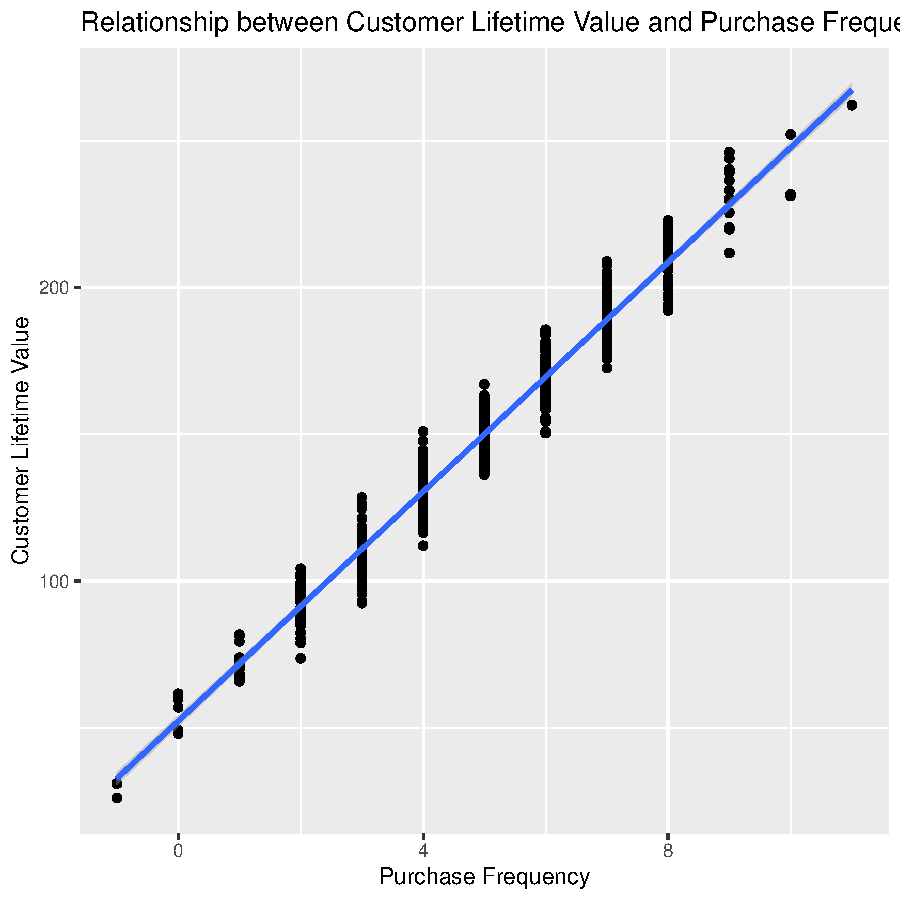
\includegraphics[keepaspectratio]{1_simple_linear_regression_files/figure-latex/scatter_plot_2-1.pdf}}

\section{Statistical Test}\label{statistical-test}

We then apply a simple linear regression as a statistical test for
regression.

\begin{Shaded}
\begin{Highlighting}[]
\NormalTok{slr\_test }\OtherTok{\textless{}{-}} \FunctionTok{lm}\NormalTok{(customer\_lifetime\_value }\SpecialCharTok{\textasciitilde{}}\NormalTok{ purchase\_frequency, }\AttributeTok{data =}\NormalTok{ clv\_data)}
\end{Highlighting}
\end{Shaded}

View the summary of the model.

\begin{Shaded}
\begin{Highlighting}[]
\FunctionTok{summary}\NormalTok{(slr\_test)}
\end{Highlighting}
\end{Shaded}

\begin{verbatim}
## 
## Call:
## lm(formula = customer_lifetime_value ~ purchase_frequency, data = clv_data)
## 
## Residuals:
##      Min       1Q   Median       3Q      Max 
## -19.1176  -5.6169  -0.0491   5.6618  20.4837 
## 
## Coefficients:
##                    Estimate Std. Error t value Pr(>|t|)    
## (Intercept)         52.2538     0.9042   57.79   <2e-16 ***
## purchase_frequency  19.5356     0.1700  114.91   <2e-16 ***
## ---
## Signif. codes:  0 '***' 0.001 '**' 0.01 '*' 0.05 '.' 0.1 ' ' 1
## 
## Residual standard error: 7.734 on 498 degrees of freedom
## Multiple R-squared:  0.9637, Adjusted R-squared:  0.9636 
## F-statistic: 1.32e+04 on 1 and 498 DF,  p-value: < 2.2e-16
\end{verbatim}

To obtain a 95\% confidence interval:

\begin{Shaded}
\begin{Highlighting}[]
\FunctionTok{confint}\NormalTok{(slr\_test, }\AttributeTok{level =} \FloatTok{0.95}\NormalTok{)}
\end{Highlighting}
\end{Shaded}

\begin{verbatim}
##                       2.5 %   97.5 %
## (Intercept)        50.47731 54.03036
## purchase_frequency 19.20159 19.86965
\end{verbatim}

\section{Diagnostic EDA}\label{diagnostic-eda}

Diagnostic EDA is performed to validate that the regression assumptions
are true with respect to the statistical test. Validating the regression
assumption in turn ensures that the statistical tests applied are
appropriate for the data and helps to prevent incorrect conclusions.

\subsection{\texorpdfstring{\ul{\textbf{Test of
Linearity}}}{Test of Linearity}}\label{test-of-linearity}

The test of linearity is used to assess whether the relationship between
the dependent variables and the independent variables is linear. This is
necessary given that linearity is one of the key assumptions of
statistical tests of regression and verifying it is crucial for ensuring
the validity of the model's estimates and predictions.

A plot of the residuals versus the fitted values enables us to test for
linearity. For the model to pass the test of linearity, there should be
no pattern in the distribution of residuals and the residuals should be
randomly placed around the 0.0 residual line, i.e., the residuals should
randomly vary around the mean of the value of the response variable.

\begin{Shaded}
\begin{Highlighting}[]
\FunctionTok{plot}\NormalTok{(slr\_test, }\AttributeTok{which =} \DecValTok{1}\NormalTok{)}
\end{Highlighting}
\end{Shaded}

\pandocbounded{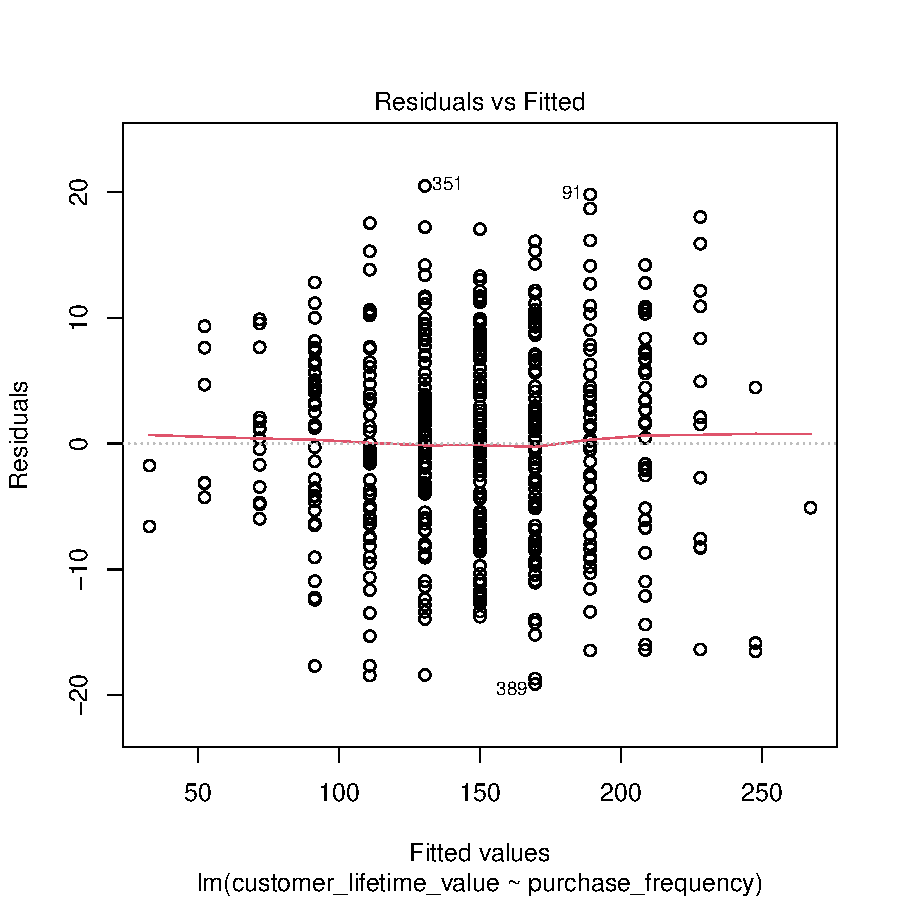
\includegraphics[keepaspectratio]{1_simple_linear_regression_files/figure-latex/test_of_linearity-1.pdf}}

\subsection{\texorpdfstring{\ul{\textbf{Test of Independence of
Errors}}}{Test of Independence of Errors}}\label{test-of-independence-of-errors}

This test is necessary to confirm that each observation is independent
of the other. It helps to identify \textbf{autocorrelation} that is
introduced when the data is collected over a close period of time or
when one observation is related to another observation. Autocorrelation
leads to underestimated standard errors and inflated t-statistics. It
can also make findings appear more significant than they actually are.

The ``\textbf{Durbin-Watson Test}'' can be used as a test of
independence of errors (test of autocorrelation).

\begin{itemize}
\item
  The null hypothesis, H\textsubscript{0}, is that there is no
  autocorrelation
\item
  The alternative hypothesis, H\textsubscript{a}, is that there is
  autocorrelation
\end{itemize}

If the p-value is greater than 0.05 then there is no evidence to reject
the null hypothesis that ``there is no autocorrelation''. The results
below show a p-value of 0.1573, therefore, the test of independence of
errors around the regression line passes.

\begin{Shaded}
\begin{Highlighting}[]
\NormalTok{pacman}\SpecialCharTok{::}\FunctionTok{p\_load}\NormalTok{(}\StringTok{"lmtest"}\NormalTok{)}
\FunctionTok{dwtest}\NormalTok{(slr\_test)}
\end{Highlighting}
\end{Shaded}

\begin{verbatim}
## 
##  Durbin-Watson test
## 
## data:  slr_test
## DW = 1.9104, p-value = 0.1573
## alternative hypothesis: true autocorrelation is greater than 0
\end{verbatim}

\subsection{\texorpdfstring{\ul{\textbf{Test of
Normality}}}{Test of Normality}}\label{test-of-normality}

The test of normality assesses whether the residuals are normally
distributed, i.e., most residuals (errors) are close to zero and large
errors are rare. A Q-Q plot can be used to conduct the test of
normality.

A Q-Q plot is a scatterplot of the quantiles of the residuals against
the quantiles of a normal distribution. Quantiles are statistical values
that divide a dataset or probability distribution into equal-sized
intervals. They help in understanding how data is distributed by marking
specific points that separate the data into groups of equal size.
Examples of quantiles include: quartiles (4 equal parts), percentiles
(100 equal parts), deciles (10 equal parts), etc.

If the points in the Q-Q plot fall along a straight line, then the
normality assumption is satisfied. If the points in the Q-Q plot do not
fall along a straight line, then the normality assumption is not
satisfied.

\begin{Shaded}
\begin{Highlighting}[]
\FunctionTok{plot}\NormalTok{(slr\_test, }\AttributeTok{which =} \DecValTok{2}\NormalTok{)}
\end{Highlighting}
\end{Shaded}

\pandocbounded{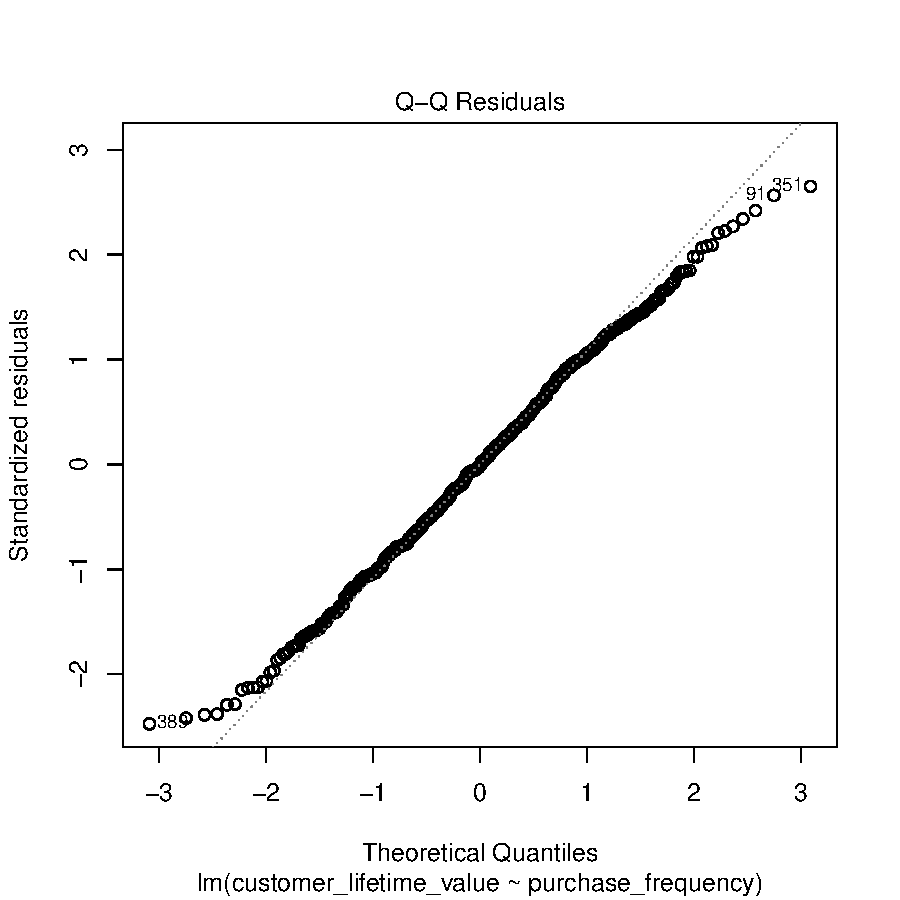
\includegraphics[keepaspectratio]{1_simple_linear_regression_files/figure-latex/test_of_normality-1.pdf}}

\subsection{\texorpdfstring{\ul{\textbf{Test of
Homoscedasticity}}}{Test of Homoscedasticity}}\label{test-of-homoscedasticity}

Homoscedasticity requires that the spread of residuals should be
constant across all levels of the independent variable. A scale-location
plot (a.k.a. spread-location plot) can be used to conduct a test of
homoscedasticity.

The x-axis shows the fitted (predicted) values from the model and the
y-axis shows the square root of the standardized residuals. The red line
is added to help visualize any patterns.

In a model with homoscedastic errors (equal variance across all
predicted values):

\begin{itemize}
\item
  Points should be randomly scattered around a horizontal line
\item
  The smooth line should be approximately horizontal
\item
  The vertical spread of points should be roughly equal across all
  fitted values
\item
  No obvious patterns, funnels, or trends should be visible
\end{itemize}

Points forming a cone shape that widens from left to right suggests
heteroscedasticity with increasing variance for larger fitted values.

\begin{Shaded}
\begin{Highlighting}[]
\FunctionTok{plot}\NormalTok{(slr\_test, }\AttributeTok{which =} \DecValTok{3}\NormalTok{)}
\end{Highlighting}
\end{Shaded}

\pandocbounded{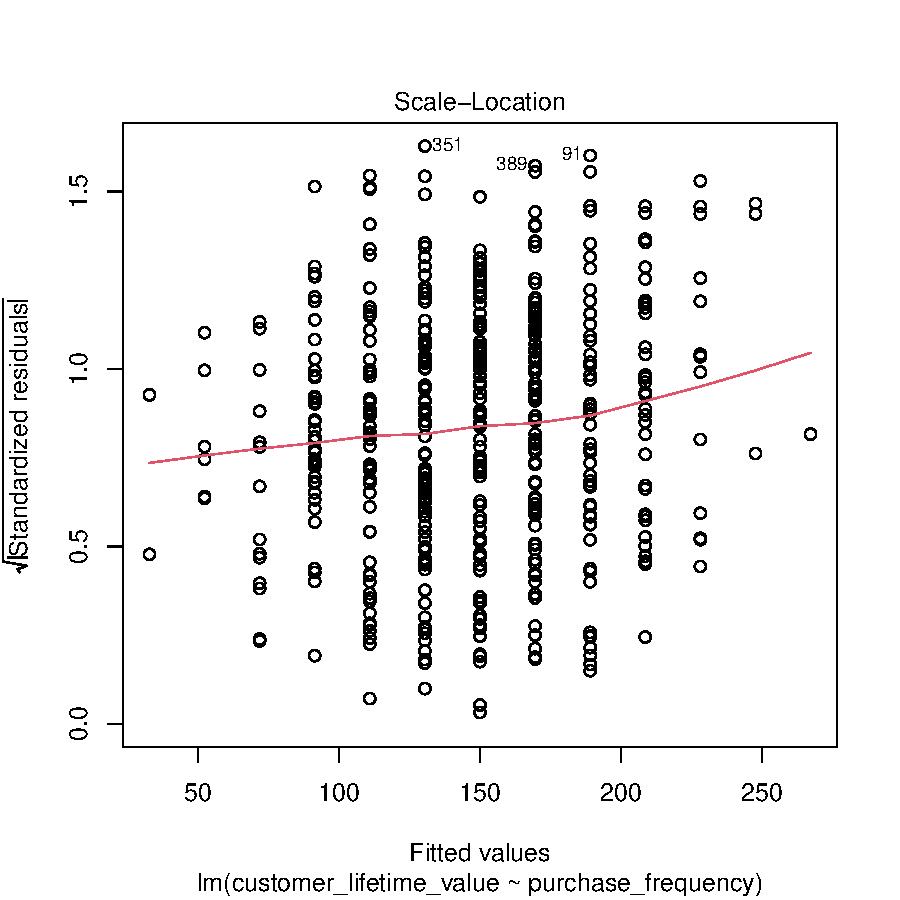
\includegraphics[keepaspectratio]{1_simple_linear_regression_files/figure-latex/test_of_homoscedasticity-1.pdf}}

\subsection{\texorpdfstring{\ul{\textbf{Quantitative Validation of
Assumptions}}}{Quantitative Validation of Assumptions}}\label{quantitative-validation-of-assumptions}

The graphical representations of the various tests of assumptions should
be accompanied by quantitative values. The \texttt{gvlma} package
(Global Validation of Linear Models Assumptions) is useful for this
purpose.

\begin{Shaded}
\begin{Highlighting}[]
\NormalTok{pacman}\SpecialCharTok{::}\FunctionTok{p\_load}\NormalTok{(}\StringTok{"gvlma"}\NormalTok{)}
\NormalTok{gvlma\_results }\OtherTok{\textless{}{-}} \FunctionTok{gvlma}\NormalTok{(slr\_test)}
\FunctionTok{summary}\NormalTok{(gvlma\_results)}
\end{Highlighting}
\end{Shaded}

\begin{verbatim}
## 
## Call:
## lm(formula = customer_lifetime_value ~ purchase_frequency, data = clv_data)
## 
## Residuals:
##      Min       1Q   Median       3Q      Max 
## -19.1176  -5.6169  -0.0491   5.6618  20.4837 
## 
## Coefficients:
##                    Estimate Std. Error t value Pr(>|t|)    
## (Intercept)         52.2538     0.9042   57.79   <2e-16 ***
## purchase_frequency  19.5356     0.1700  114.91   <2e-16 ***
## ---
## Signif. codes:  0 '***' 0.001 '**' 0.01 '*' 0.05 '.' 0.1 ' ' 1
## 
## Residual standard error: 7.734 on 498 degrees of freedom
## Multiple R-squared:  0.9637, Adjusted R-squared:  0.9636 
## F-statistic: 1.32e+04 on 1 and 498 DF,  p-value: < 2.2e-16
## 
## 
## ASSESSMENT OF THE LINEAR MODEL ASSUMPTIONS
## USING THE GLOBAL TEST ON 4 DEGREES-OF-FREEDOM:
## Level of Significance =  0.05 
## 
## Call:
##  gvlma(x = slr_test) 
## 
##                      Value p-value                Decision
## Global Stat        5.08943 0.27824 Assumptions acceptable.
## Skewness           0.03973 0.84201 Assumptions acceptable.
## Kurtosis           3.61252 0.05735 Assumptions acceptable.
## Link Function      0.01459 0.90385 Assumptions acceptable.
## Heteroscedasticity 1.42258 0.23298 Assumptions acceptable.
\end{verbatim}

\section{Interpretation of the
Results}\label{interpretation-of-the-results}

We can interpret the results of the statistical test with more
confidence if the tests of assumptions are successful.

\subsection{Academic Statement}\label{academic-statement}

A simple linear regression was conducted on data from 500 observations
(N = 500) to examine the relationship between customer lifetime value
(CLV) and purchase frequency. The results indicated that purchase
frequency significantly predicted CLV, \(\beta\) = 19.54, 95\% CI
{[}19.20, 19.87{]}, SE = 0.17, \emph{t}(498) = 114.91, \emph{p}
\textless{} .001. The model explained 96.37\% of the variance in CLV
(R\textsuperscript{2} = .96, \emph{F}(1, 498) = 13,200, \emph{p}
\textless{} .001). For every unit increase in purchase frequency, CLV
increased by approximately 19.54 units. The intercept was 52.25, 95 \%
CI {[}50.48, 54.03{]}, and the residual standard error was 7.73,
indicating strong predictive accuracy.

\subsection{Business Analysis}\label{business-analysis}

The strength of the relationship highlights the critical importance of
customer retention. Initiatives that effectively encourage repeat
purchases appear to be a primary driver of customer lifetime value based
on this analysis. This understanding can guide the allocation of
resources towards strategies that foster customer loyalty and encourage
repeat business.

\subsection{Limitations}\label{limitations}

The model employed is a simple linear regression, which only considers
the linear relationship between purchase frequency and CLV. Other
potentially influential factors that are not included in this model
could also play a significant role in determining CLV, e.g., the average
monetary value of each purchase.

\end{document}
